\chapter{Contexto}
\thispagestyle{fancy}
\fancyhead[LE]{\thechapter.Contexto} 
En el siguiente capítulo se introducirán y explicarán los conceptos importantes sobre los que parte el proyecto. Es de gran importancia comprender y conocer lo que son los sistemas de recomendación y el Federated Learning para entender tanto el desarrollo, como la resolución de los problemas y retos que supone su implementación. 

\section{Sistemas de recomendación}
Los sistemas de recomendación se basan en una gran cantidad de datos para generar predecciones. En el caso de que el sistema de recomendación fuera el de una tienda, este buscaría correlación entre los usuarios y los tipos de productos que compran, para así, recomendar ciertos artículos al grupo de personas que sea más probable que los compren.
\\ \\
A la hora de realizar la recomendación se aplican “filtros” de diferente índole, entre los más comunes se encuentran:
\begin{itemize}
    \item Filtros demográficos, que recomiendan en función del sexo, edad, país, oficio, … 
    \item Filtros basados en contenidos, como Youtube, que recomiendan contenidos similares a los valorados por los usuarios. 
    \item Filtrado colaborativo, que consiste en recomendar al usuario elementos valorados positivamente por usuarios similares a él. 
\end{itemize}

Sin embargo, existen sistemas híbridos que utilizan varias de las estrategias de filtrado anteriores combinadas. Un ejemplo de ello es Amazon, que tiene uno de los algoritmos de recomendación más potentes. 
\\ \\
Esto se debe a dos cosas, en primer lugar que cuenta con una gran cantidad de información de los usuarios, tanto su edad, género, país, dirección, rutinas (si tienen Alexa), … como los artículos que miran, compran, añaden a la lista, etc. El algoritmo es capaz de ofrecer recomendaciones muy precisas a los usuarios y dar una gran calidad de servicio gracias a esto.
\\ \\
De hecho, en Amazon, si queremos revisar las recomendaciones tenemos un apartado propio para ellas al que se puede acceder fácilmente (Fig\ref{fig:AmazonRecomendaciones}).
 
\begin{figure}[thbp]
    \centering
    \fbox{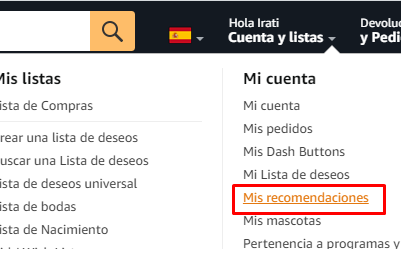
\includegraphics[width=0.45\textwidth]{Figuras/Amazon_acceder_mis_recomendaciones.png}}
    \fbox{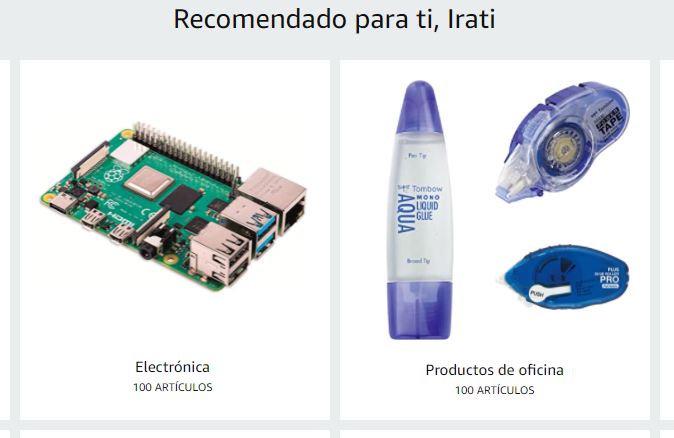
\includegraphics[width=0.45\textwidth]{Figuras/Amazon_recomendaciones.png}}
    \caption{Recomendaciones de Amazon (Fuente: Amazon\autocite{AmazonEsCompra})} 
    \label{fig:AmazonRecomendaciones}
\end{figure}

\section{Federated Learning}
El aprendizaje federado, o Federated Learning en inglés, es una rama del Machine Learning que busca entrenar al algoritmo a través de diversos dispositivos descentralizados, manteniendo siempre la información en cada uno de ellos. Estos dispositivos descentralizados forman una red de aprendizaje colaborativo que busca mejorar la precisión del algoritmo mediante la combinación de los modelos de cada participante de la red en un servidor central

\begin{figure}[thbp]
    \centering
    \fbox{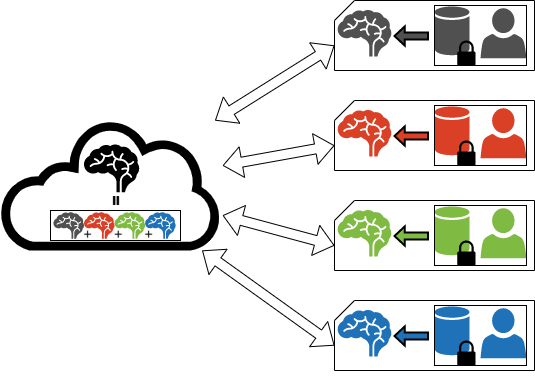
\includegraphics[width=0.45\textwidth]{Figuras/FedLeaConcept.png}}
    \caption{Diagrama de una red de Federated Learning} 
    \label{fig:FedLearArquitectura}
\end{figure}
Al contrario del machine learning, que reunía toda la información en un mismo computador, el aprendizaje federado busca entrenar un algoritmo en cada uno de los dispositivos que participen en la red para luego combinar estos algoritmos. Una vez combinados son mandados de vuelta a los participantes de la red para poder mejorarlos y que estos sean más precisos gracias a la información de otros participantes.